\documentclass{article}
\usepackage[UTF8]{ctex}
\usepackage{amsthm}
\theoremstyle{definition}
\newtheorem{theorem}{定理}
\newtheorem{example}{例}
\newtheorem{definition}{定义}
\newtheorem{lemma}{引理}
\newtheorem{proposition}{命题}
\newtheorem{corollary}{推论}
\newtheorem{jie}{解}
\theoremstyle{remark}
\newtheorem{rem}{补充说明}
\theoremstyle{theorem}
\newtheorem{ques}{问题}
\usepackage{yfonts}
\usepackage{titlesec}
\usepackage{tabularx}
\usepackage{ltxtable}
\usepackage{diagbox}
\usepackage{amstext}%公式中加入文字
\usepackage{graphicx} %插入图片的宏包
\usepackage{float} %设置图片浮动位置的宏包
\usepackage{subfigure} %插入多图时用子图显示的宏包
\usepackage{mathtools}
\usepackage{listings}
\usepackage{float}
\usepackage{makecell}
\usepackage{colortbl}
\usepackage{xcolor}
\usepackage{array}
\usepackage{latexsym}
\usepackage{amsfonts}
\usepackage{amssymb}
\usepackage{textcomp}
\usepackage{booktabs}
\usepackage{epigraph}
\usepackage{amssymb,dsfont}
\usepackage{amsbsy}
\usepackage{enumerate}
\usepackage{flowchart}
\title{Tebac 暑期讲义}
\author{邓志远 }
\date{\today}

\begin{document}

\maketitle
\textbf{数学目标:准备应用题,基础数列问题,几何拼接面积等问题,三个主题。重点在于准备相关数学词汇的法语词汇。讲义中有部分内容是希望同学们课下去阅读,自己去探索,并不要求一定学会。}
\textbf{The Goal of English Courses: We want to communicate with students in English by games, presentations, or small theater. }

\section{第一周数学:几何图形的面积}
\subsection{认识图形与对称}
首先认识各种图形:正方体图形见图\ref{eye}:
\begin{example}
\begin{figure}
    \centering
    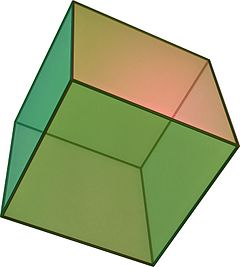
\includegraphics[scale=0.3]{Cube.jpg}
    \caption{正方体}
    \label{fig:my_label}
\end{figure}
\end{example}
\begin{definition}
对称轴:图形沿着此直线对折,两侧可以完全重合,则称这条直线为对称轴。

中心对称:以某个点为中心,图形旋转180度后,可以与自身重合,则称之为中心对称图形。
\end{definition}
中心对称图形的例子:
\begin{example}
\begin{figure}
    \centering
    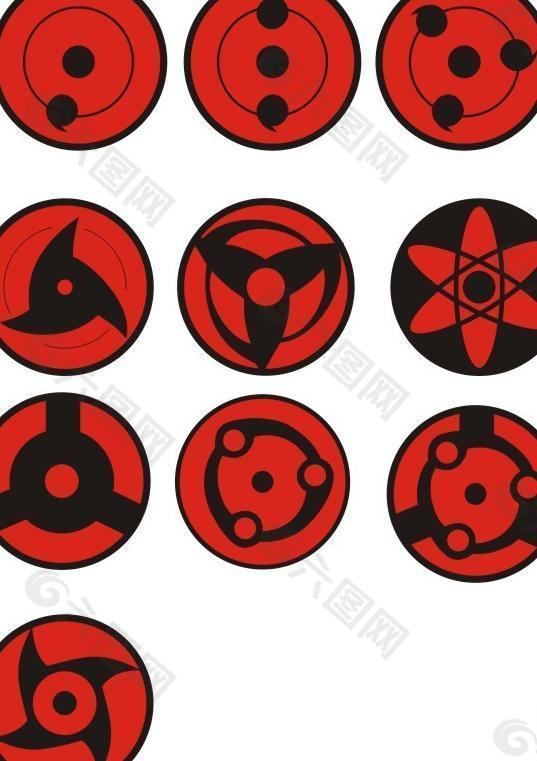
\includegraphics[scale=0.3]{eye.jpg}
    \caption{中心对称}
    \label{eye}
\end{figure}
\end{example}
这部分设置练习题为判断给定图形的对称与否,并数对称轴数量。
\subsection{面积的计算}
正方形的面积公式:$\textbf{边长}^{2}$;
正方形的周长公式:4$\times\textbf{边长 }$;
\begin{figure}
    \centering
    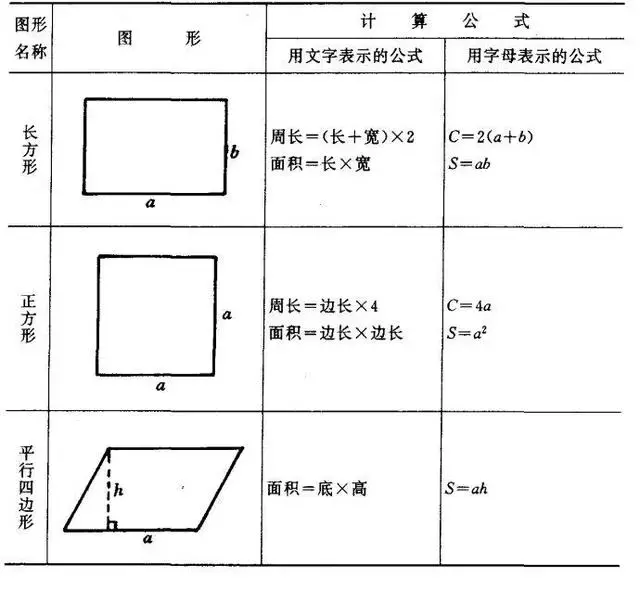
\includegraphics[scale=0.5]{area.png}
    \caption{图形的面积与周长}
    \label{fig:my_label}
\end{figure}
\begin{figure}
    \centering
    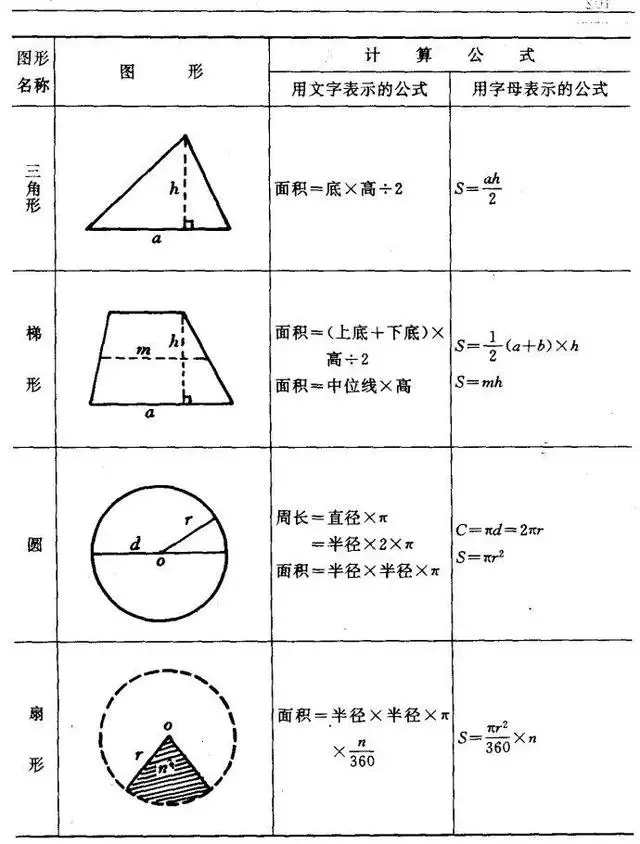
\includegraphics[scale=0.5]{area2.png}
    \caption{图形的面积与周长}
    \label{fig:my_label}
\end{figure}

这部分对于学生的难点在于想明白圆面积公式的由来,详见图\ref{fig:circle},把圆一步一步切开,然后拼接成一个矩形(长方形)。这里用到了“近似”的思想(极限)。
\begin{figure}
    \centering
    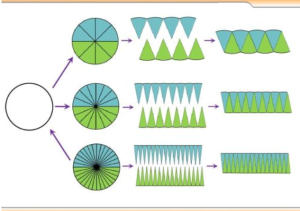
\includegraphics{circle.jpg}
    \caption{圆面积公式的由来}
    \label{fig:circle}
\end{figure}
另外需要去理解圆周率是如何得来的:世界上最早把圆周率精确计算到小数点后7位是中国祖冲之,如图\ref{zuchongzhi}
\begin{figure}
    \centering
    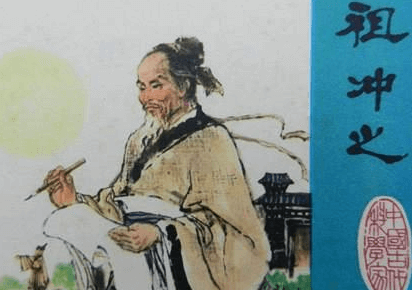
\includegraphics[scale=0.5]{zuchongzhi.jpg}
    \caption{祖冲之}
    \label{zuchongzhi}
\end{figure}
圆周率是通过多边形不断近似得到,计算方式如图\ref{pi}。
\begin{figure}
    \centering
    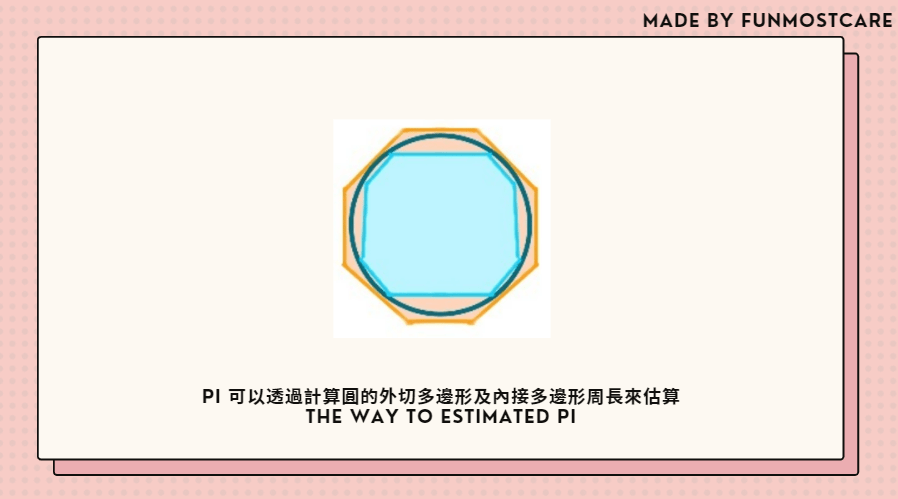
\includegraphics[scale=0.3]{pi-estimate.png}
    \caption{圆周率的计算}
    \label{pi}
\end{figure}
\section{The lecture of first week: English}
The first English is mainly about asking questions. By the games "who is the spy" and the guess game, students have to practice asking question to each other.

The format of question is very simple: is it.... or are you....? During the games, students have to ask each other and defense themselves. For example, given an object on the board, then the student have to repeat the format of questions, which is very efficient way to practice the basic sentence.
\section{第一周科学}
第一周的科学课解释了两个生活中最常见的东西:水和空气。

通过解释水的分子结构:$H_{2}O$,重点希望让学生们明白科学的发展史:不断问为什么,不断的犯错。课堂中鼓励学生不断问为什么,也回答了学生们各种各样千奇百怪的问题:为什么人生出来人,不是生出来其他动物?时间又没有尽头?光是什么?等等。这是一个很有趣的探索的过程。

第二部分内容解释了大气强是什么。解释压强是什么:
\begin{equation*}
    P(\textbf{压强})=\frac{F(\textbf{受力})}{S(\textbf{接触面积})}
\end{equation*}
然后通过解释了汽车上安全锤的科学原理,解释了“怎么打人比较痛”。

流体力学在生活中 的应用:速度越大,压强越小。通过这样的原理解释了火车月台安全险的原理。
\section{第二周:鸡兔同笼以及方程}
随堂测试,复习加减乘除,分数,小数,百分数的运算。
\begin{rem}
    2+3=5        Deux et trois font cinq. Ou
             Deux plus trois égale/égalent cinq.
             
5-3=2        Cinq moins trois égale/égalent deux.

2*3=6        Deux fois trois égale/égalent six.

6/3=2        Six devisé par trois égale/égalent deux.

1,5   un virgule cinq

99,9  quatre-vingt-dix-neuf virgule neuf

3\%    trois pour cent

50\%   cinquante pour cent

100\%  cent pour cent
\end{rem}

\begin{ques}[鸡兔同笼]
    鸡(poulet)兔(lapin)同笼,首十,脚二八,问鸡有几只,兔子有几只。
\end{ques}
我们希望通过画图,列表等等,比较有趣的方法,来引入方程。
\begin{jie}[画图法]
\begin{enumerate}
    \item 画10个圆圈表示10个头:
    \item 给每个头下添上2只脚,见图\ref{fig:head-foot}:
    \begin{figure}
        \centering
        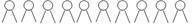
\includegraphics{head-foot.png}
        \caption{头}
        \label{fig:head-foot}
    \end{figure}
    \item 发现总脚数比题目中的少,说明有兔子,则再一次添上兔腿,直到脚的数量和题目中的一致:
    \begin{figure}[H] %H为当前位置,!htb为忽略美学标准,htbp为浮动图形
\centering %图片居中
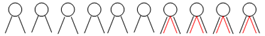
\includegraphics[width=0.7\textwidth]{jitu.png} %插入图片,[]中设置图片大小,{}中是图片文件名
\caption{圆圈代表头,斜线为腿} %最终文档中希望显示的图片标题
\label{jitu} %用于文内引用的标签
\end{figure}
\end{enumerate}
\end{jie}
\begin{jie}[列表法]
请同学自己将表格完成:
\begin{center}
    \begin{tabular}{c|c|c}
    鸡(只) & 兔(只)& 总共有多少只脚 \\
    1 & 9 & 38\\
    2 & 8 & \\
    3 & 7 & \\
    4& 6 & \\
    5 & 5 & \\
    6 & 4 & \\
    7 & 3 & \\
    8 & 2 & \\
    9 & 1 & 
\end{tabular}
\end{center}
\end{jie}
\begin{jie}[假设法或置换法]

如果10只都是兔子,一共应该有$4\times 10=40$只脚,这和已经知道的28只脚相比多了40-28=12只脚。如果用一个只鸡来代替一只,就要减少4-2=2只脚。那么,10只兔子应该用几只鸡来代替,从而使得12只脚的差值没有了呢?也就是说:12/2=6,只要用6只鸡来代替6只兔子就行了。所以,鸡的只数就是6只,兔子就应该是4只了。

友情提示:同学们发现了嘛?假设对象和你先求出的对象是相反的。

那么反过来呢?如果我们假设一共有10只鸡呢?

\end{jie}
\begin{jie}[抬腿法或者坐下法]
\begin{enumerate}
    \item 抬腿法:鸡有两条腿,兔子有四条腿,2和4都是偶数(même)。想象如果各自去掉一半,这样每只鸡变成了只有一只腿,兔子还剩下两只腿,总脚数就是28/2=14,兔子:14-10=4,鸡:10-4=6。
    
    提示:同学们有没有办法用画图法来画出来这个呢?
    \item 坐下法:想象一下如果鸡和兔子抬起2条腿,那么鸡一屁股就坐在了地上了。但是兔子可以站着。一共抬起来了 $2\times10=20$条腿,剩下了28-20=8条腿,全是兔子,则兔子有8/2=4,所以鸡是10-4=6只。
    
    这个方法可以找同学们来表演一下。
\end{enumerate}
补充:偶数(même),奇数(nombre impair),素数(nombre premier)。
\end{jie}
\begin{jie}[方程法]
这是最重要的做法!!!!

在这个方法之前,需要向同学们解释什么是这个神秘的“$x$”.


假设鸡一共有x只,兔子一共有(10-x)只:
那么
一共 28只脚:
$$2x+4(10-x)=28$$
解出来我们得到:$x=6$.

也就是说一共有6只鸡,4只兔子。

这个$x$的运算性质与数字相同,需要花时间解释这个“运算性质”是什么。
对于理解快的同学,可以二元一次方程:
假设鸡为$x$只,兔子有$y$只:
所以我们可以得到两个方程:

\begin{align*}
\text{头:}x+y=10;\\
\text{脚:}2x+4y=28.
\end{align*}

\end{jie}
\begin{ques}
    有蜘蛛(araignée),蜻蜓(libellule),蝉(cigale)三种动物,共有腿118对,翅膀(aile)20对。问蜻蜓有多少只?
    
    注:蜘蛛8条腿,蜻蜓有6条腿,两对翅膀。蝉有6条腿,一对翅膀。
\end{ques}
\begin{ques}[马拉瓦]
    100匹马,100块瓦,大马驮三,中马驮俩,小马俩驮一个,问有多少大马、中马和小马?
\end{ques}
\section{The lecture of second week English course}
The goal for second week is to practice about Past tense. 

By using "I did..." or "what did you do", student have to repeat these kinds of format of sentences.

The practice is by using the game known as the werewolf or Mafia. In the game, there are six roles avilable for students: the god, the doctor, the seer, the hunter and the werewolf and the villager. The god is in charge of asking questions and help the process of the game. 

The first stage of the game is the night: the god will guide the game: 
\begin{enumerate}
    \item werewolves wake up and who would you want to kill?
    \item Doctor wake up, who would you want to heal?
\end{enumerate}
The other roles procede in the same manner. The most important part for our courses is to use simple past tense to explain what they did last night. So this is a nice game, at the same time it's useful to repeat the past tense to practice it. 
\section{第二周科学:水}
虹吸作用(Siphon (tuyau)):
Une extrémité du siphon (entrée) est placée dans le récipient supérieur. Le siphon doit être rempli de liquide, soit avant la mise en place, soit par un amorçage consistant à créer une dépression (par aspiration) qui permet au liquide du réservoir de s'engager dans le tuyau.

Lorsque l'autre extrémité (sortie) du tuyau est descendue à un niveau inférieur au niveau du réservoir, le liquide s'écoule. L'énergie nécessaire au mouvement est celle de la chute du liquide entre le niveau du réservoir supérieur et la hauteur du tuyau de sortie s'il est à l'air libre, ou le niveau d'un réservoir inférieur, si le tuyau y plonge. La profondeur à laquelle se trouve l'extrémité d'entrée n'intervient pas (tant qu'elle reste plongée dans le liquide).

Si le niveau de sortie est remonté plus haut que celui du liquide dans le réservoir supérieur, le mouvement s'inverse et le siphon se désamorce si de l'air peut s'y introduire à la place du liquide.

Souvent, on parle de "siphonnage" d'essence lorsqu'une personne cherche à vider son réservoir.

连通器(Communicating vases):
En mécanique des fluides, le principe des vases communicants établit qu'un liquide homogène remplissant plusieurs récipients, reliés entre eux à leur base et soumis à la même pression atmosphérique, s'équilibre à la même hauteur dans chacun d'eux. Ceci est vrai quels que soient leur forme et leur volume. Si le même liquide ou un liquide de même densité est ajouté dans l'un des récipients, il va à nouveau s'équilibrer à une hauteur identique dans tous les récipients connectés.

毛细现象(Capillarité):La capillarité est le phénomène d'interaction qui se produit aux interfaces entre deux liquides non miscibles, entre un liquide et l'air ou entre un liquide et une surface. Elle est due aux forces de tension superficielle entre les différentes phases en présence. Elle est mise en œuvre lorsque les buvards aspirent l’encre, les éponges s’imbibent d’eau, ou quand on trempe une partie de son morceau de sucre dans son café et que ce sucre devient tout noir.
\section{第三周}
\subsection{第三周数学:数的分类}
\textbf{目标:理解什么是负数,掌握负数的运算规则,理解什么是无理数。对于感兴趣的同学,可以尝试自主学习什么是勾股定理,通过勾股定理(毕达哥拉斯Pythagoras定理),理解$\sqrt{2}$的诞生。}

数的分类:

首先第一种分类:我们可以将数字分成正数,0,负数。

第二种比较抽象的分类:有理数和无理数。有理数中包含了整数,比如3,有限小数,比如0.2,无限循环小数,比如$\frac{2}{3}=0.666...$. 无理数中是无限不循环小数,比如$\pi$见图\ref{fig:piirr}.
\begin{figure}
    \centering
    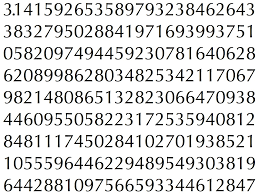
\includegraphics{piirr.png}
    \caption{圆周率}
    \label{fig:piirr}
\end{figure}
历史上无理数最著名的例子便是$\sqrt{2}$,这部分内容属于选择性学习内容。

正数就是我们从小时候便熟悉的数。负数的概念最直接的例子就是借钱:我从某位同学那里借了5元钱,我可以记录为“欠某某同学5元”或者简单的写为“-5”来表示我借钱了。对于负数的乘法:我们可以理解为多次借钱,借了一次-5,又借一次,又一次,总共就是$-5\times 3$.



\subsection{English Lecture for Third Week}
\textbf{The goal for English this week is to understand the }
\section{第四周}
\section{第五周}

\end{document}
